\documentclass[12pt]{article}
\usepackage[english]{babel}
\usepackage[utf8x]{inputenc}
\usepackage[T1]{fontenc}
\usepackage{scribe}
\usepackage{listings}
\usepackage{graphics, graphicx}
\usepackage{enumitem}
\usepackage{tcolorbox}
\usepackage{adjustbox}
\usepackage{algorithm}
\usepackage[english]{babel}
\usepackage{amsthm}
\usepackage[noend]{algpseudocode}
\usepackage{tikz}
\usepackage{forest}
\usepackage{mathtools}
\usepackage{amsthm}
\usepackage[noend]{algpseudocode}
\usepackage{wasysym}
\forestset{
	sn edges1/.style={for tree={edge={->},where n children=0{tier=word}{}}}, 
	background tree/.style={for tree={text opacity=0.2,draw opacity=0.2,edge={draw opacity=0.2}}},
	sn edges2/.style={for tree={edge={<-},where n children=0{tier=word}{}}},
}

\graphicspath{ {./images/} }

\newcommand{\epz}{\epsilon > 0}
\newcommand{\dez}{\delta > 0}
\newcommand{\nat}{\mathbb{N}}
\newcommand{\real}{\mathbb{R}}
\newcommand{\rational}{\mathbb{Q}}
\newcommand{\integer}{\mathbb{Z}}
\newcommand{\nthroot}[2]{\sqrt[\leftroot{-2}\uproot{2}#1]{#2}}
\newcommand{\eneighbourhood}[2]{V_{#1} (#2)}
\newcommand{\inv}{^{-1}}
\newcommand*{\lsim}{\mathord{\sim}}

\newcommand{\whp}{\textit{w.h.p.}}
\newcommand{\expected}{\mathbb{E}}
\newcommand{\probab}{\mathbb{P}}
\newcommand{\normdist}[2]{\mathcal{N}(#1,#2)}

\CourseName{Comtemporary Algorithms T.II/2019-20}
\Scribe{Kriangsak T. \& Apivich H.}
\Lecturer{Dr. Kanat Tangwongsan}
\LectureNumber{17}
\LectureDate{4 March 2020}
\LectureTitle{Gradient Descent \& SGD}

\lstset{style=mystyle}

\newlist{steps}{enumerate}{1}
\setlist[steps, 1]{label = Step \arabic*:}

\algblock{ParFor}{EndParFor}
\algnewcommand\algorithmicparfor{\textbf{parfor}}
\algnewcommand\algorithmicpardo{\textbf{do}}
\algnewcommand\algorithmicendparfor{\textbf{end\ parfor}}
\algrenewtext{ParFor}[2]{\algorithmicparfor\ #1\ \textbf{in}\ #2 \algorithmicpardo}
\algrenewtext{EndParFor}{\algorithmicendparfor}

\tikzset{every picture/.style={line width=0.75pt}} %set default line width to 0.75pt      

\begin{document}
\MakeScribeTop

\section{Convex Functions}

First, we have to define the notion of convexity. The formal definition of convex sets are as follows.

\begin{definition}
	A set $K$ is \textit{convex} if for all $x, y \in K$, $\lambda x + (1-\lambda) y \in K$ for all $\lambda \in [0, 1]$. 
\end{definition}

Geometrically, a set is convex if any line between any two points in the set does not leave the set. Note that in the definition above, $\lambda x + (1-\lambda) y$ can be thought of as a line connecting two points $x$ and $y$ together.

\begin{figure}[H]
	\centering
	
\includegraphics[width=0.3\linewidth]{img1}
\end{figure}


From here, we can define convex functions as follows.

\begin{definition}
	A function $f: \real^n \to \real$ is convex if for any $x, y \in \real^n$, $f(\lambda x + (1-\lambda)y) \leq \lambda f(x) + (1-\lambda) f(y)$ for all $\lambda \in [0, 1]$. 
\end{definition}

We can imagine this in 2D space. Geometrically, if you draw a line from $(x, f(x))$ to $(y, f(y))$, then the line will always be ``above" the function. We can also say that the region above the function (or the set $\{(x, y) \in \real^2 : f(x) \leq y\}$ if in 2D) is a convex set.

\begin{figure}[H]
	\centering
	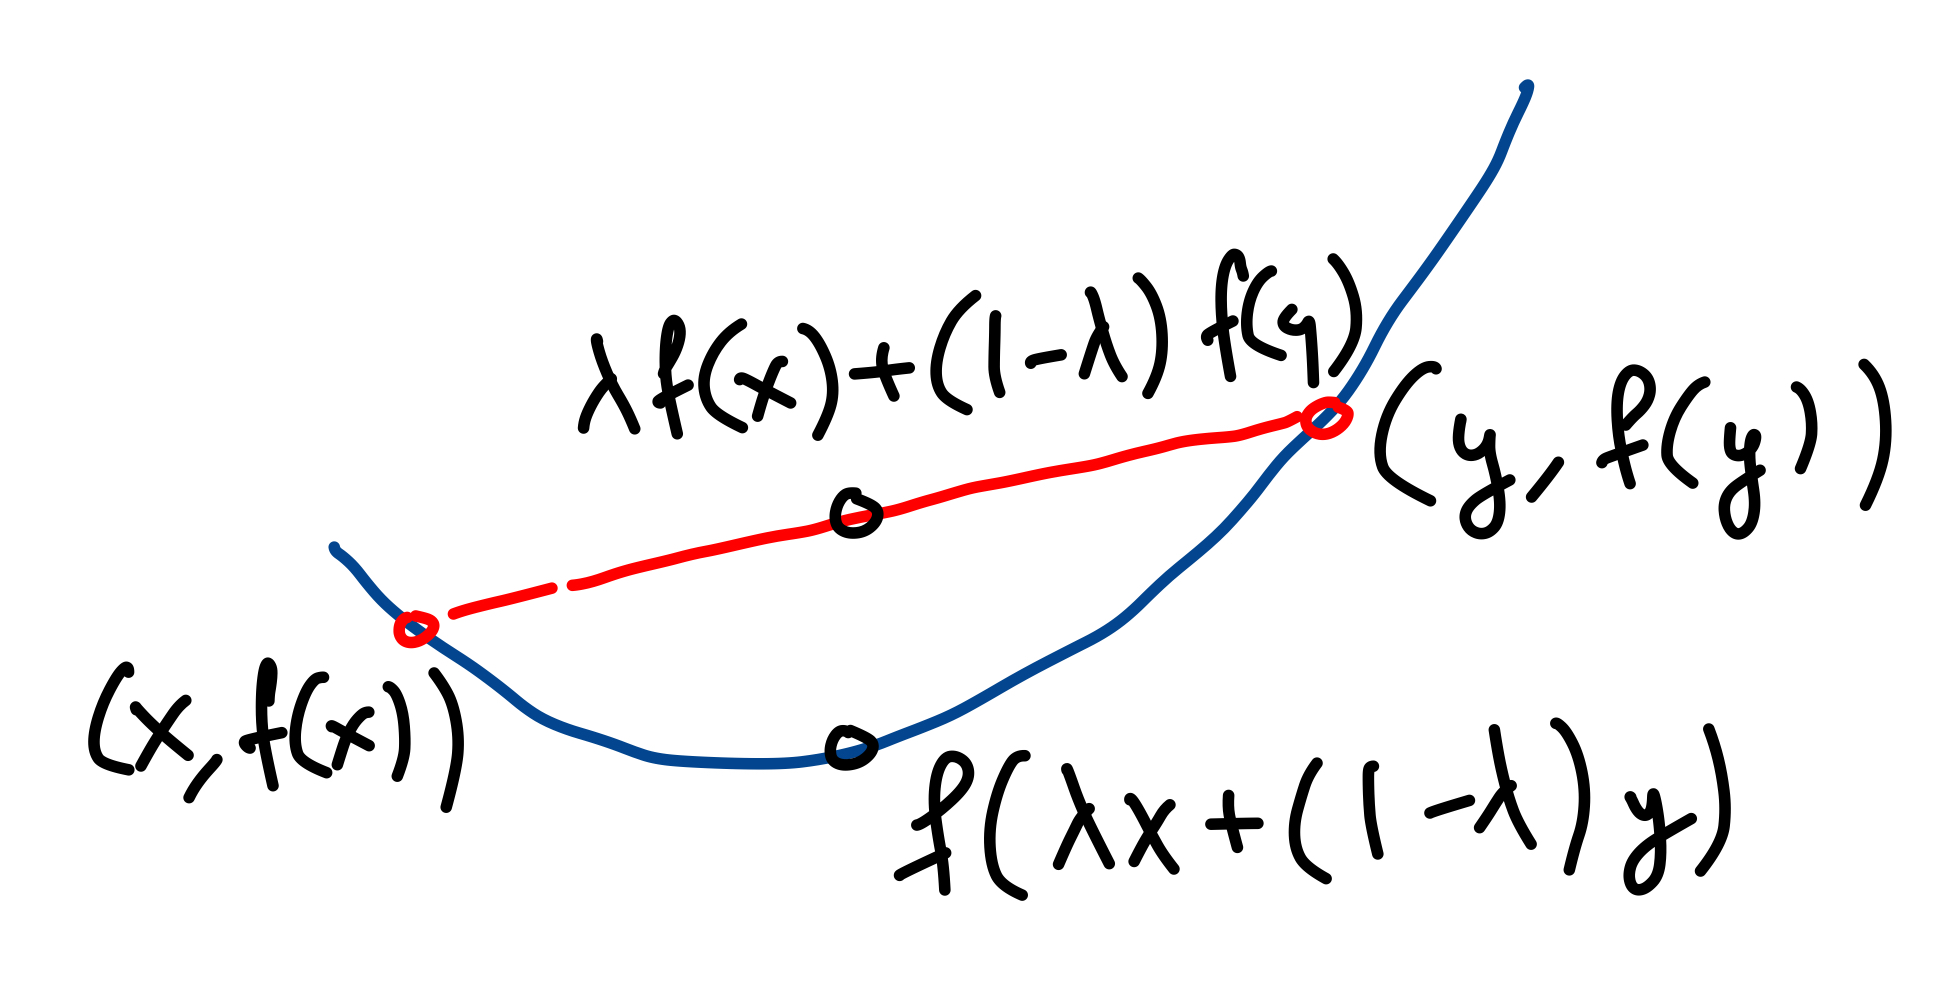
\includegraphics[width=0.4\linewidth]{img2}
\end{figure}

A useful result about differentiable convex functions is the following.
\begin{fact}
	For differentiable convex function $f$, $f(y) \geq f(x) + \nabla f(x)^T (y-x)$. 
\end{fact}
This is simply due to the fact that for convex function, the graph always will be curving away, so approximating the function using a straight line will always give a lower value than in reality. Note that here we have used the symbol $\nabla$ (or the gradient operator), which is the way to generalise the derivative to higher dimensions. 

\begin{figure}[H]
	\centering
	
\includegraphics[width=0.4\linewidth]{img3}
\end{figure}

We can also define something called the Hessian matrix as the following.
\begin{definition}
	For twice-differentiable function $f$, we can define the \textit{Hessian matrix} as $Hf$, where $$(Hf)_{ij} = \frac{\partial^2f}{\partial x_i \partial x_j}.$$ 
\end{definition}
We can also determine the convexity of a function by its Hessian matrix.
\begin{fact}
	A twice-differentiable function $f$ is convex if and only if its Hessian matrix $Hf$ is positive semidefinite for all $x$ (i.e. the eigenvalue of $Hf$ is always positive).
\end{fact}

Finally, we will define the notion of a function being $\lambda$-Lipschitz.
\begin{definition}
	A function $f: \real^n \to \real$ is $\lambda$-Lipschitz if for all $x, $ in $\real^n$, $\|f(x) - f(y) \| \leq \lambda \|x-y\|_2$. 
\end{definition}
Intuitively, $\lambda$-Lipschitz functions are functions which doesn't change too rapidly. If you travel some distance $d$ away from a point, then you would expect the function to only change by $\lambda d$ amound at most (we won't use this definition in this lecture, but we'll define it anyway).

\section{Gradient Descent}

\subsection{The Problem}

After much definitions, we will now define the problem that we want to solve. In this lecture, we are given a convex function $f: \real^n \to \real$, and we would like to find some $x^* \in \real^n$ which will give the lowest possible value of $f(x^*)$. 

From early calculus classes, this is a simple task as we know the minimum point must be such that $\nabla f(x^*) = 0$. However, this is not always easy to find. An example of such is if we consider the function $$f(x) = \frac{1}{2}x^TAx - b^Tx,$$ we can see that $\nabla f(x) = Ax - b$, and to find where $\nabla f(x) = 0$ means finding the solution to $Ax = b$, which is not necessarily easy. We will therefore come up with a different method to do this.

\subsection{Gradient Descent Algorithm}

The idea is we can try to ``walk" to the solution. We can start with some initial guess of the minimum, and pick the next value we should walk to. We see that given some value, we should walk to the point which is lower down. This corresponds to walking in the direction of $-\nabla f$. We can keep walking until we reach the minimal point.

We can express the algorithm as the following.
\begin{algorithm}[H]
	\caption{Gradient Descent Algorithm}
	\begin{algorithmic}[1]
		\Function{GradientDescent}{$f, x_0$}
		\For{$t = 1, 2, \ldots, T$}
			\State {$x_t \gets x_{t-1} - \eta_t \nabla f(x_{t-1})$}
		\EndFor
		\State \Return $\hat{x} = \frac{1}{T} \sum_{t} x_t$
		\EndFunction
	\end{algorithmic}
\end{algorithm}
The algorithm requires the function $f$ which we want to optimise. We also need some initial starting point $x_0$ which starts off the iterations. In the end, we take the mean of all the steps that the algorithm walks to.

Note that we also have the parameter $\eta_t$ which is known as the step size. This determines how big each of the steps will be. There is no good rule for what it should be, but  a step size too slow and the solution converges slowly, but a step size too big and you will keep ``stepping over" the actual solution. 

\begin{figure}[H]
	\centering
	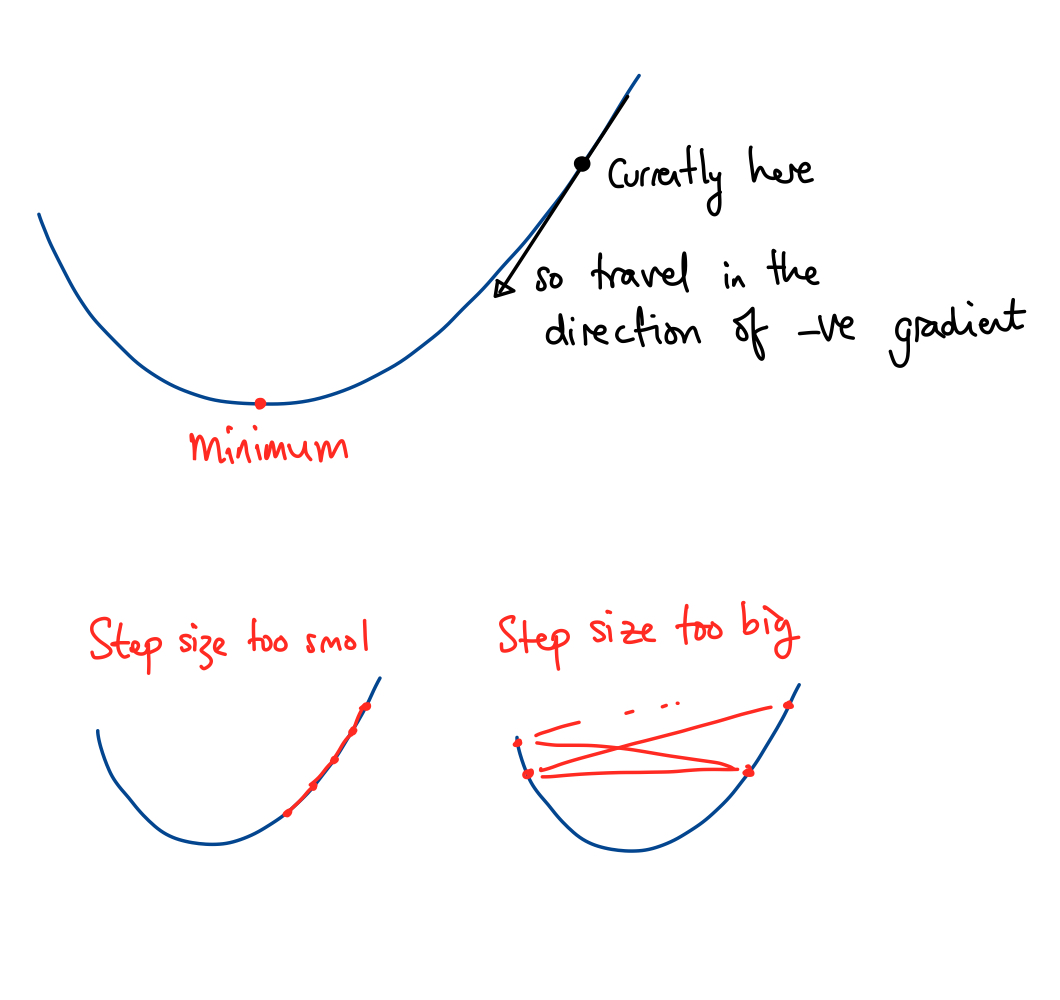
\includegraphics[width=0.6\linewidth]{img4}
\end{figure}

\subsection{Analysis}

We can now try to quantitatively describe the performance of the Gradient Descent algorithm. We make the following claim about the algorithm.
\begin{theorem}
	\label{gdthm}
	Let $x^*$ be the minimiser of $f : \real^n \to \real$. If $f$ is convex and differentiable and satisfies $\|\nabla f(x)\|_2 \leq G$ for all $x\in\real^n$, then setting $T = \frac{G^2}{\epsilon^2}\|x_0 - x^*\|_2^2$ and $\eta_t = \eta = \frac{\|x_0 - x^*\|}{G\sqrt{T}}$ gives $f(\hat{x}) \leq f(x^*) + \epsilon$. 
\end{theorem}
\begin{proof}
	To prove the theorem, we will use the fact (which will be proven later in Lemma \ref{gdlma}) that 
	$$\sum_{t} f(x_t) \leq Tf(x^*) + \frac{1}{2}G^2T\eta + \frac{1}{2\eta}\|x_0 - x^*\|_2^2.$$ 
	We can see that
	\begin{align*}
		f(\hat{x}) &= f\bigg( \frac{1}{T}\sum_{t} x_t\bigg) \\
		&\leq \frac{1}{T}\sum_{t}  f( x_t) &\text{by convexity of $f$}\\
		&\leq f(x^*) + \frac{1}{2}G^2\eta + \frac{1}{2T\eta}\|x_0 - x^*\|_2^2 &\text{by above} \\
		&= f(x^*) + \frac{G}{\sqrt{T}} \|x_0 - x^*\|_2 &\text{by our choice of $\eta$} \\
		&= f(x^*) + G\|x_0 - x^*\|_2 \sqrt{\frac{\epsilon^2 \|x_0 - x^*\|_2^2}{G^2}} &\text{by our choice of $G$} \\
		&=f(x^*) + \epsilon
	\end{align*}
	which proves our theorem.
\end{proof}
An interesting observation from the proof above is that we can see that from Line 4 of the maths above, $f(\hat{x}) \leq f(x^*) + \frac{G}{\sqrt{T}} \|x_0 - x^*\|_2$, i.e. $f(\hat{x}) - f(x^*) \leq O(\frac{1}{\sqrt{T}})$. This roughly shows that the error in our solution goes down proportional to $\frac{1}{\sqrt{T}}$. 

We now have one more thing that we need to prove from above. 
\begin{lemma}
	\label{gdlma}	
	Let $f$ and $x^*$ be defined as we have done in Theorem \ref{gdthm}. Then, $$\sum_{t} f(x_t) \leq Tf(x^*) + \frac{1}{2}G^2T\eta + \frac{1}{2\eta}\|x_0 - x^*\|_2^2.$$
\end{lemma}
\begin{proof}
	Let $\Phi_t = \frac{1}{2\eta} \|x_t -x^*\|_2^2$. Then, we can see that
	\begin{align*}
		f(x_t) + \Phi_{t+1} - \Phi_t &= f(x_t) + \frac{1}{2\eta} \bigg( \|x_{t+1} -x^*\|_2^2 -  \|x_t -x^*\|_2^2\bigg) \\
		&= f(x_t) + \frac{1}{2\eta} \bigg( (x_{t+1} -x^*)^T (x_{t+1} -x^*) -  (x_{t} -x^*)^T (x_{t} -x^*)\bigg).
	\end{align*}
	Let $\Delta x_t = x_{t+1} - x_t$ and $y = x_t - x^*$. Then, 
	\begin{align*}
	f(x_t) + \Phi_{t+1} - \Phi_t &= f(x_t) + \frac{1}{2\eta} \bigg( (\Delta x_t + y)^T(\Delta x_t + y) -y^Ty \bigg) \\
	&= f(x_t) + \frac{1}{2\eta} \bigg( \|\Delta x_t\|^2 + 2\Delta x^Ty\bigg).
	\end{align*}
	However, we know that $\Delta x_t = x_{t+1} - x_t = -\eta \nabla f(x_t)$, and so
	\begin{align*}
			f(x_t) + \Phi_{t+1} - \Phi_t &= f(x_t) + \frac{1}{2\eta} \bigg( \eta^2 \|\nabla f(x_t)\|^2 + 2\nabla f(x_t)^Ty\bigg) \\
			&\leq \frac{1}{2}G^2 \eta + \underbrace{f(x_t) - 2f(x_t)^T(x_t - x^*)}_\text{$\leq f(x^*)$ by the property of convex functions} \\
			&\leq \frac{1}{2}G^2 + f(x^*)
	\end{align*}
	We have shown that $f(x_t) + \Phi_{t+1} - \Phi_t \leq \frac{1}{2}G^2 + f(x^*)$. From this, we can therefore see that
	\begin{align*}
		\sum_{t} f(x_t) &= \sum_{t=1}^{T} [f(x_t) + \Phi_t - \Phi_{t-1}] - \Phi_T + \Phi_0 \\
		&\leq \sum_{t=1}^{T} [f(x_t) + \Phi_t - \Phi_{t-1}] + \frac{1}{2\eta}\|x_0 - x^*\|_2^2 &\text{definition of $\Phi_t$, and since $\Phi_T \geq 0$} \\
		&\leq Tf(x^*) + \frac{1}{2}TG^2 + \frac{1}{2\eta}\|x_0 - x^*\|_2^2 &\text{from above}
	\end{align*}
	which proves our lemma.
\end{proof}

\subsection{Remarks}
\begin{itemize}
	\item[(i)] What the heck is $ \eta \nabla f(x)$ ?
	The second-order Taylor's expansion :
	$$
	f(y) \approx f(x) + f'(x)\cdot (\vec{y}-\vec{x}) + \frac{1}{2} f''(x)(\vec{y}-\vec{x})^2 
	$$  
	In $ d \geq 2$,
	$$
	f(\vec{y}) \approx f(\vec{x} + \nabla f(\bar{x})^T(\vec{y}-\vec{x}) +\frac{1}{2}(\vec{y}-\vec{x})^T \nabla^2f(x)(\vec{y}-\vec{x}) 
	$$
	where $\nabla^2f(x)$ is Hessian $Hf(k)$. This potentially complex $Hf$ can be approximated by an extremely simple term $\frac{1}{\eta}I$, where $I$ is the identity matrix. That is,
	$$
	\tilde{f}(\vec{y}) = f(\vec{x}) + \nabla f(\bar{x})^T(\vec{y}-\vec{x}) +\frac{1}{2\eta}||\vec{y}-\vec{x}||_2^2
	$$ 
	This turns out to be convex for some complex reasons. The question now is how to minimize $\tilde{f}(\vec{y}) $?. To do this, by convexity, set$ \nabla{y} \tilde{f}(\vec{y})  =0$. Then,
	$$
	\nabla{y} \tilde{f}(\vec{y})  =  \nabla f(\vec{x}) + \frac{1}{\eta}(\vec{y}-\vec{x}) =0 \Longleftrightarrow \vec{y} -\vec{x} = -\frac{1}{\eta} \nabla f(\vec{x}) 
	$$ 
	This technique is called \textit{\textbf{minimization of local approximations}} where $f +\nabla$ is local approximation and $\frac{1}{2\eta}||\vec{y}-\vec{x}||$ is proximity. 
	\item[(ii)] In practice,  how to  choose $\eta_t$? Fixing $\eta_t$ throughout an approximation is not always a good idea. Therefore, a popular heuristic is to have a decaying $\eta_t$
	\item[(iii)] For further refinement, for instance,  the function $f$ needs to be \textit{strongly} convex (i.e.,  the function must "bend"). 
\end{itemize}

\section{Stochastic Gradient Descent}

\subsection{Special Case Popular in Machine Learning/Deep Learning}
\begin{itemize}
	\item In machine learning, we will often want to minimise a loss function $f(\vec{\theta}) = \frac{1}{n} \sum_{i=1}^{n} f_i(\vec{\theta})$ with $\vec{\theta}$ being some model parameter.
	\item Example: In linear regression with $l_2$ loss. Data points $(\vec{x_{i,j}},y_i)$ where $y_i$ is a label. The loss function is given by, 
	$$
	\text{loss} =\sum_{i=1}^{n} (y_i - \vec{x_i}^T \vec{\theta})^2
	$$
	Minimizing this loss function is equivalent to minimizing 
	$$
	f(\vec{\theta})= \frac{1}{n}\sum_{i=1}^{n} (y_i - \vec{x_i}^T \vec{\theta})^2
	$$ 
	\item Notice that running GD takes $O(nd)$ per iteration. This is too costly, there shall be a way to reduce this.
	\item Fun fact: $\mathbb{E}_i [f_i(\vec{\theta)}] = f_i(\vec{\theta)}$ and $\nabla_{\theta} f_i(\vec{\theta)} = \frac{1}{n}\sum_{i=1}^{n} f_i(\vec{\theta)}$
	This fact gives rise to Stochastic Gradient Descent (SGD) whereby space requirement and time complexity per iteration is reduced. 
\end{itemize}

\subsection{SGD Algorithm}

We can express the algorithm as the following.
\begin{algorithm}[H]
	\caption{Stochastic Gradient Descent Algorithm}
	\begin{algorithmic}
		\Function{GradientDescent}{$f, x_0$}
		\For{$t = 1, 2, \ldots, T-1$}
		\State choose  an $i$ at random or round robin.
		\State {$x_t \gets x_{t-1} - \eta_t \nabla f_i(x_{t-1})$}
		\EndFor
		\State \Return $\hat{x} = \frac{1}{T} \sum_{t} x_t$
		\EndFunction
	\end{algorithmic}
\end{algorithm}
We can also state a similar bound proof as before.
\begin{theorem}
	\label{sgdthm}
	Let $x^*$ be the minimiser of $f : \real^n \to \real$. If $f$ is convex and differentiable and satisfies $\|\nabla f_i(x)\|_2 \leq G$ for all $x\in\real^n$, then setting $T = \frac{G^2}{\epsilon^2}\|x_0 - x^*\|_2^2$ and $\eta_t = \eta = \frac{\|x_0 - x^*\|}{G\sqrt{T}}$ gives $\mathbb{E}f(\hat{x}) \leq f(x^*) + \epsilon$. 
\end{theorem}
This is the same old proof. The interesting bits are: 
\begin{claim}
	Let $\Phi_t = \frac{1}{2 \eta} \|x_t -x^*\|_2^2$.
	Then, $ \mathbb{E} \bigg [f(\vec{x_t}  + (\Phi_{t+1} - \Phi_t) \bigg ] \leq f(x^*) + \frac{1}{2} \eta G^2 $
\end{claim}
Condition $\mathbb{E}$ on the history until iteration that produced $\vec{x_t}$
\begin{align*}
\mathbb{E} [ f( \vec{x_t})  + \Phi_{t+1} - \Phi_t ] &\leq \mathbb{E} \bigg[f(\vec{x_t}) + \frac{1}{2} \eta  \bigg (|| \underbrace{ \vec{x_{t+1}} - \vec{x_t}}_{ \Delta x } ||_2^2 + 2\Delta x^T(\vec{x_t} -x^*) \bigg ) \bigg ]\\
&\leq \mathbb{E}[f(\vec{x_t}] + \frac{1}{2} \eta  G^2 - \nabla f(\vec{x})^T(\vec{x_t} -x^*) \\
&= \frac{1}{2} \eta  G^2 + \underbrace{f(\vec{x_t}) +\nabla f(\vec{x})^T(x^* +\vec{x_t} }_{\leq f(x^*))}  
\end{align*}
Note: 
\begin{align*}
\Delta x &= -\eta f_i(\vec{x_t})\\
&\Rightarrow || \Delta x||_2^2 \leq \eta^2 G^2\\
&\Rightarrow \mathbb{E}_i[\Delta x] = -\eta \mathbb{E}[\Delta_{f_i}(\vec{ x_t}] = -\eta	\Delta f(\vec{x_t})
\end{align*}
Other tricks used to implement SGD: 
\begin{itemize}
	\item $\mathbb{E}_i [f_i(\vec{x})] = f_i(x) $ but potentially \underline{not} concentrated (i.e. high variance). Therefore, This potentially does not converge as fast as performing the full gradient. 
	\item To improve further, Pick a "batch" of indices. Say, $B \leq [n]$ and use an update rule such that
	$$
	\vec{x_t} = \vec{x_{t-1}} - \frac{\eta}{|B|} \sum_{i \in B} \nabla f_i(\vec{x_{t-1}}).
	$$
	Note: $ \mathbb{E}\bigg[ \frac{1}{|B|}\cdot \sum_{i \in B} \nabla f_i(\vec{x})\bigg] = \frac{1}{|B|}\sum_{i \in B}  \nabla f_i(\vec{x} )=\nabla f(\vec{x} ) $
\end{itemize}
By doing this, minibatch sampling, the variance is reduced by about $\frac{1}{|B|}$ and the cost per iteration shrinks down to $O(|B|\cdot d)$. This is considered a good compromise in practice since the convergence rate, (i.e.,$f(\hat{x}) -f(x^*)$), is  $O\bigg(\sqrt{\frac{|B|}{T} + \frac{|B|}{T}} \bigg)$as opposed to $O\big(\frac{1}{T} \big)$ in a normal GD algorithm.

\end{document}
